\documentclass{sig-alternate-05-2015}
%-------------------- Packages --------------------%

\documentclass[11pt,a4paper]{report}
\usepackage[utf8]{inputenc}
\usepackage[french]{babel}
\usepackage[T1]{fontenc}
\usepackage{amsmath} %pour les formules maths
\usepackage{amsfonts}
\usepackage{amssymb}
\usepackage{graphicx} %pour inclure des images
\usepackage{hyperref} %pour les lien URLs
\usepackage[left=2cm,right=2cm,top=3cm,bottom=3cm]{geometry}
\usepackage{pifont} %pour les puces spéciales
\usepackage{listings} %pour écrire du code
\usepackage{xcolor} %pour la mise en couleur
\usepackage{multirow} %pour les tableaux
\usepackage{bclogo} %pour des boîtes texte avec un logo


%-------------------- New Colors --------------------%

%Basic

\definecolor{purple}{rgb}{0.6, 0.2, 0.9}

%Dark
\definecolor{dkgreen}{rgb}{0,.6,0}
\definecolor{dkblue}{rgb}{0,0,.6}
\definecolor{dkyellow}{cmyk}{0,0,.8,.3}
\definecolor{dkred}{rgb}{0.6, 0, 0}


%Light
\definecolor{ltblue}{rgb}{0.67, 0.85, 0.9}
\definecolor{ltred}{rgb}{0.8, 0.32, 0.32}
\definecolor{ltgrey}{rgb}{0.94,0.94,0.94}



%-------------------- Config lstlisting --------------------%

\lstset{
language=php,
basicstyle=\ttfamily\tiny, %
identifierstyle=\color{dkred}, %
keywordstyle=\color{dkblue}, %
stringstyle=\color{dkgreen}, %
commentstyle=\it\color{gray}, %
emph=[1]{php},
emphstyle=[1]\color{black},
emph=[2]{if,and,or,else},
emphstyle=[2]\color{dkyellow},
emph=[3]{imap_open, imap_close, imap_fetch_overview, imap_check, imap_list, imap_mail_move, imap_search, imap_fetchstructure			},
emphstyle=[3]\color{dkblue},
emph=[4]{string, int, double, float, private, public, static, bool, resource, array, object},
emphstyle=[4]\color{purple},
columns=flexible, %
tabsize=2, %
extendedchars=true, %
showspaces=false, %
showstringspaces=false, %
numbers=left, %
numberstyle=\tiny, %
breaklines=true, %
breakautoindent=true, %
captionpos=b, %
backgroundcolor=\color{ltgrey}
}

\makeatletter
\def\@copyrightspace{\relax}
\makeatother

\begin{document}
%General Information
\setcopyright{acmcopyright}
\title{La biométrie par reconnaissance faciale}
%\subtitle{Analyse et découverte d'une technologie}
\numberofauthors{1}
\author{
Wéry Benoît\\
       \affaddr{ECAM - 1e Master Informatique}\\
       \affaddr{1200 Bruxelles, Belgique}\\
       \affaddr{\today}\\
}
\maketitle

\begin{abstract}
%Prévoir 1 page (2 colonnes) pour Abstract + Introduction + Conclusion -> reste seulement 3 pages (6 colonnes)
\textit{
A travers cet article seront passés en revue le concept de biométrie et l'une de ses techniques les plus courante: la reconnaissance de visage.\\Les notions élémentaires de biométrie seront expliquées pour mieux comprendre le contexte dans lequel s'inscrit le processus de reconnaissance et différentes méthodes seront ensuite brièvement présentées pour mettre en avant les nombreuses possibilités de traitement d'une image contenant un visage ainsi que l'usage de la reconnaissance faciale dans notre quotidien.}
\end{abstract}

\section{Introduction}
%\textit{Bref rappel historique, motivations, utilité, ... Présentation du découpage de l'article}
Si la reconnaissance de visages est une tâche complètement anodine pour le cerveau humain, il n'en va pas de même pour les systèmes informatiques. Bien au contraire, ce processus s'avère être un réel défi technologique mélangeant techniques de capture d'images et algorithmes de traitements. \\
Pourtant, la reconnaissance faciale automatique est très appréciée en tant que technique biométrique et utilisée dans de nombreuses applications. C'est pourquoi, depuis la fin des années 1970, les travaux de recherches ont permis de mettre au point de nouvelles méthodes qui se sont succédées et améliorées avec le temps pour passer de simples processus de traitement 2D à des systèmes capables d'analyser un visage en 3D et en temps réel, le tout dans des systèmes de plus en plus miniaturisés.
\paragraph{}
Alors, quelle est la place de la reconnaissance faciale par rapport aux différentes techniques biométriques existantes? Quelles sont les méthodes les plus connues et quelles applications les utilisent?\\ C'est ce que nous tenterons de découvrir à travers cet article.
\paragraph{}
Dans un premier, la notion de biométrie sera expliquée ainsi que le fonctionnement général des systèmes biométriques. On verra également pourquoi il est intéressant d'utiliser des caractéristiques de l'être humain pour améliorer les aspects de sécurité d'un système.
\\
Ensuite, la reconnaissance faciale sera présentée en suivant la logique de ses trois étapes caractéristiques, à savoir: la \textit{détection}, la \textit{normalisation} et la \textit{reconnaissance 2D et 3D}.
\\
Enfin, deux exemples seront présentés pour mettre en avant des cas d'utilisation différents des systèmes biométriques par reconnaissance de visage: la détection et l'authentification.
\section{La biométrie}
%\textit{Une donnée est dite biométrique si elle permet l'identification d'une personne sur base de ce qu'elle est, qu'il s'agisse d'une caractéristique physiologique ou comportementale. Ainsi, on peut parler du visage comme étant une donnée biométrique.}
La biométrie, qui signifie "mesure du vivant", désigne dans notre contexte \textit{"l'ensemble des procédés de reconnaissance d'une personne par certaines de ses caractéristiques physiques ou comportementales"}.\cite{Xmisc_3}. Il s'agit donc d'utiliser des informations, telles que: l'empreinte digitale, l'iris, le visage, la démarche, ... afin de pouvoir identifier ou confirmer l'identité d'un sujet humain.
%\begin{itemize}
%\item[$\cdot$]\textsc{universelles} - peuvent être analyser sur chaque individu
%\item[$\cdot$]\textsc{uniques} - sont différentes pour chaque individu
%\item[$\cdot$]\textsc{invariables} - ne changent que très peu, voir pas du tout, au cours du temps
%\item[$\cdot$]\textsc{enregistrables} - peuvent être stockées de façon numérique
%\item[$\cdot$]\textsc{mesurables} - peuvent être comparées
%\end{itemize}

\subsection{Systèmes biométriques}
%\textit{Les composants principaux et les différents modes (enrôlement, identificaiton, authentification)}
Un système biométrique fonctionne sur la comparaison de deux fichiers, issus de données biométriques, afin de déterminer leur taux de similitude.
\\
Dans un tel système, une première phase dite d'\textit{enrôlement} permet de récupérer la donnée et de l'enregistrer de façon numérique en BDD sous forme d'un modèle mathématique, que l'on appelle \textit{"signature"} ou \textit{"gabarit"}. On distingue ensuite deux modes de comparaison des modèles (voir \ref{id-vs-auth}): 
\begin{itemize}
\item[$\cdot$]l'\textsc{authentification} - comparaison 1:1
\item[$\cdot$]l'\textsc{identification} - comparaison 1:N
\end{itemize}
\begin{figure}[h!]
\includegraphics[scale=.45]{images/systeme-biometrique.png}
\caption{Modules d'un système biométrique}
\end{figure}

\subsection{Aspects sécurité}
Les systèmes biométriques sont particulièrement appréciés pour augmenter la sécurité des processus de vérification.
\\En effet, un code PIN ou un mot de passe peuvent être facilement trouvés selon leur niveau de complexité. Les données biométriques, quant à elles, présentent les avantages suivants, elles sont: universelles, uniques, invariables, enregistrables et mesurables.
\\Ainsi, leur utilisation complique le piratage ainsi que l'usurpation d'identité. De plus, un système biométrique ne nécessite plus de retenir un code. Pour ces raisons, ils sont de plus en plus utilisés dans les processus qui nécessitent la vérification de l'utilisateur.

\subsection{Critères de performances et comparaison des technologies}
Les éléments essentiels qui déterminent la qualité d'un tel système sont: la \textit{donnée}, le \textit{capteur} - nécessité d'obtenir un modèle analysable de bonne résolution - et les \textit{algorithmes} (détection, analyse, comparaison).
%\textit{Intrusivité, fiabilité, coût, effort -> la place du visage d'en tout ça...}
\paragraph{}
Toutes les caractéristiques biométriques exploitables ne se valent pas mais elles peuvent être comparées selon différents critères tels que: l'\textit{intrusivité}, la \textit{fiabilité}, le \textit{coût} ou encore l'\textit{effort} (contribution du sujet lors de son analyse).
\paragraph{}
Ainsi, par exemple, si les empreintes digitales et l'iris sont meilleures que la reconnaissance du visage en termes de performances, cette dernière technique, quant à elle, est jugée moins intrusive et moins contraignante pour l'utilisateur. En effet, elle ne nécessite pas la coopération du sujet car il peut être identifié à distance. De plus les capteurs utilisés peuvent être relativement bons marché, puisqu'il s'agit dans le plus simple des cas d'un appareil photo ou d'une caméra.
\\Néanmoins, comme nous allons le voir, la reconnaissance faciale est sujette à diverses contraintes qui compliquent l'obtention d'une information de qualité et son analyse.

\subsection{Evaluation de la fiabilité}
Comme cela a été dit, un système biométrique évalue le taux de similitude entre deux modèles pour authentifer un individu. Or, il est impossible d'obtenir une coïncidence de 100\% entre deux signatures. Dès lors, il faut fixer des seuils d'acception, qui permettent de quantifier les performances d'un système selon les facteurs suivants \cite{Xmisc_2}:
\begin{itemize}
\item[$\cdot$]\textsc{TFR} - Taux de Faux Rejets : pourcentage d'individus rejetés alors qu'ils devraient être acceptés
\item[$\cdot$]\textsc{TFA} - Taux de Fausses Acceptation : pourcentage d'individus acceptés alors qu'ils devraient être rejetés
\item[$\cdot$]\textsc{TEE} - Taux d'Egale Erreur : point d'équivalence des erreurs. Il s'agit de l'intersection des deux autres courbes, qui est utilisée pour mesurer la performance de l'algorithme.
\end{itemize}
 (voir annexe \ref{perfo-systeme} pour les courbes)
\section{La reconnaissance faciale}
%\textit{Présentation de qqes résultats fondamentaux sur des recherches en cognition et reconnaissance faciale du visage}
La reconnaissance faciale est une des techniques utilisables dans les systèmes biométriques d'authentification \textit{(ex: contrôle d'accès)} ou d'identification \textit{(ex: surveillance d'un lieu)}.
\\
Plusieurs méthodes peuvent être appréhendées pour la capture de l'image, cela va dépendre principalement du contexte: il peut s'agir d'un système statique ou bien dynamique, d'une reconnaissance 2D ou 3D, ... Les capteurs de l'information et les algorithmes doivent être choisis en conséquence.

\subsection{Détection de visage}
Après avoir capturé la donnée à analyser, dans ce cas-ci une image ou une vidéo, la première étape consiste à en extraire l'information utile. Plusieurs méthodes permettent de détecter des visages dans une image, elles peuvent être regroupées en quatre catégories \cite{Xthesis_1}
\begin{enumerate}
\item \textit{Knowledge-based methods}: basées sur la connaissance des éléments caractéristiques d'un visage (\textit{nez, bouche, yeux,...}) et des relations entre eux, pour déterminer si les positions relatives décrivent un visage ou non. Malheureusement, ces techniques ont un faible taux de détection.
\item \textit{Feature invariant approaches}: basées sur des éléments invariants tels la signature de couleur de la peau ou les caractéristiques du visages. Un algorithme classique est celui de \textit{De Silva} qui consiste à trouver l'axe des yeux et utiliser ensuite comme référence la longueur entre le haut du visage et le plan de l'oeil.
\item \textit{Template matching methods}: basées sur l'utilisation de templates, pour calculer la corrélation entre l'image candidate et un template. Un modèle est défini à partir d'un certains nombre de relations "essentielles" et "de confirmation". Un visage est alors localisé lorsque le nombre de relations détectées dépassent un certains seuil.
\item \textit{Appearance-based methods}: basées sur la connaissance de modèles obtenus par apprentissage automatique. On retrouve ici un algorithme fréquemment utilisé, celui de \textit{Viola et Jones}, qui utilise un nombre considérable de modèles exemples, représentants la variabilité de l'aspect facial. Il analyse l'image de façon itérative, en agrandissant sa fenêtre de recherche en pixels, pour y retrouver des visages.
\end{enumerate}
\paragraph{}
Plusieurs difficultés se présentent lors de cette étape et compliquent la localisation du visage. En effet, les conditions de capture de l'image peuvent varier, les éléments suivants rentrent donc en compte:
%il n'est pas toujours garantit d'obtenir 
\begin{itemize}
\item[$\cdot$]la \textit{pose}: fait varier l'orientation du visage
\item[$\cdot$]les \textit{occultations}: le visage peut être partiellement ou complètement caché par certains objets
\item[$\cdot$]les \textit{expressions faciales}: engendrent la déformation du visage et donc des variations de posistions des éléments caractéristiques
\item[$\cdot$]la \textit{luminosité}: les conditions d'éclairage et les ombres qui en résultent peuvent affecter l'aspect du visage.
\item[$\cdot$]la \textit{présence ou absence de composantes structurales}: telles que la barbe, la moustache, les lunettes,...
\end{itemize}

\subsection{Prétraitement ou normalisation}
Une fois le visage détecté dans l'image, l'étape de prétraitement va permettre de rendre cette photo exploitable en la ramenant à un format prédéfini. Ainsi, toutes les images auront une taille, une échelle et des couleurs normalisées, ce qui est essentiel pour garantir les performances de la reconnaissance \cite{Xthesis_1}.
\\
Deux processus sont importants pour préparer l'image:
\begin{enumerate}
\item normalisation \textsc{géométrique}: permet de positionner et redimensionner la taille du visage
\item normalisation \textsc{photométrique}: consiste à jouer sur les niveaux de l'illumination du visage, par exemple, en augmentant les nuances pour améliorer le contraste.
\end{enumerate}


\subsection{Reconnaissance 2D}
L'étape de reconnaissance permet d'extraire de l'image les informations qui serviront à la création d'une signature numérique et, par la suite, la comparaison avec les modèles en BDD.
Les techniques qui permettent la reconnaissance de données à partir d'une image 2D peuvent être regroupées en trois familles \cite{Xphdthesis_1}
\begin{enumerate}\setlength{\itemsep}{.3em}
\item Approches \textsc{\textbf{globales}}: le visage tout entier est utilisé et représenté par un vecteur de grande dimension.
\\L'avantage de ces méthodes est qu'elles permettent de conserver toutes les informations du visage et peuvent donc tenir compte des aspects de l'organisation globale de celui-ci. 
\\Cependant, elles utilisent uniquement des images 2D, qui sont d'autant plus sensibles au critères cités précédemment (\textit{pose, illumination, expression,...}), et l'espace occupé par ces vecteurs est assez contraignant. \paragraph{}Il est alors possible d'utiliser des techniques de réduction de la dimension, telles que:
	\begin{itemize}\setlength{\itemsep}{.2em}
	\item[$\cdot$]\textit{\textbf{A}nalyse en \textbf{C}omposantes \textbf{P}rincipales (ACP)}: dont une des méthodes les plus connues est l'\textit{Eigenfaces} qui calcule les propriétés du visage à partir de combinaisons de vecteurs propres issus des modèles dans différentes nuances de gris.
	\item[$\cdot$]\textit{\textbf{A}nalyse \textbf{D}iscriminante \textbf{L}inéaire (ADL)}
	\end{itemize}
\item Approches \textsc{\textbf{locales}}: le visage est ici représenté par un ensemble de vecteurs de dimensions plus faibles. Il existe deux grandes catégories de techniques:
	\begin{itemize}
	\item[$\cdot$] \textit{basées sur les point d'intérêts}: consistent à identifier des points particuliers du visage pour ensuite en déterminer les caractéristiques. Une méthode reconnue est l'\textit{\textbf{E}lastic \textbf{B}unch \textbf{G}raph \textbf{M}atching (EBGM)} qui consiste à créer un réseaux pour modéliser les relations entre les points d'intérêts. On obtient ainsi un graphe topologique (fig \ref{raphe-topo}).

	\item[$\cdot$] \textit{basées sur l'apparence du visage}: le visage est divisé en plus petites régions, desquelles on extrait les caractéristiques locales.
	\end{itemize}
\item Approches \textsc{\textbf{hybrides}}: techniques qui utilisent les caratéristiques locales et globales.
	\begin{figure}[h!]
	\center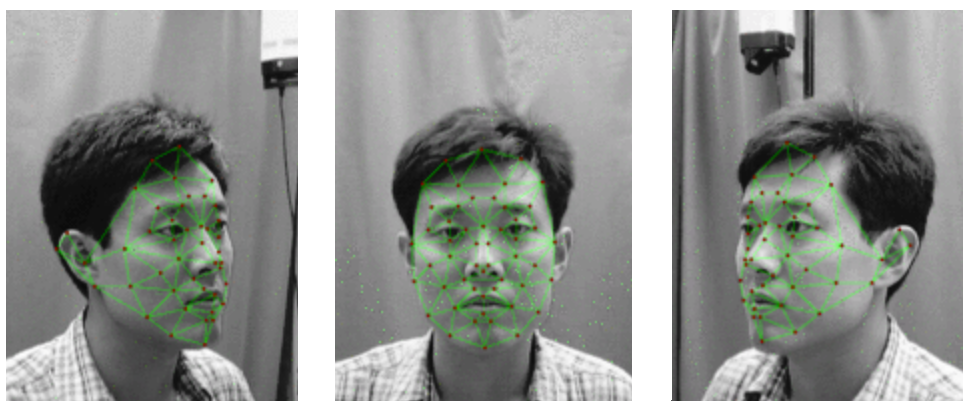
\includegraphics[scale=.3]{images/ebgm}\label{graphe-topo}
	\caption{Graphe topologique par EBGM \cite{Ximage_1}}
	\end{figure}
\end{enumerate}

De manière générale, les méthodes locales sont plus performantes et surtout moins sensibles aux changements de l'environnement, qui surviennent lors de la capture d'image (voir appendice \ref{locales-vs-globales}).


%\textit{Exploitation des caractéristiques extraites, création d'une signature numérique et mise en correspondance avec les modèles de la DB ou le modèle est vérifié\paragraph{}
%Difficultés: causes inter-sujets (ressemblance entre modèles) et intra-sujet (ci-dessus)}

\subsection{Reconnaissance 3D}
Contrairement aux techniques 2D qui viennent d'être présentées, les technologies de reconnaissance 3D permettent d'introduire la notion de \textit{profondeur} dans les images analysées. De telles techniques sont en plein essors et très prometteuses quant à leurs performances.
\\
Si les méthodes de reconnaissance sont différentes de la 2D, il en va de même pour les informations traitées et donc pour les capteurs utilisés qui ne sont plus de simples caméras. 
\\En effet, pour reconstruire un visage en 3D (\textit{par maillage polygonal par exemple}), un matériel spécial est nécessaire tel que des caméras à vision stéréoscopique ou des scans 3D à vision active. La première catégorie utilise plusieurs caméras qui sont positionnées à des endroits bien spécifiques par rapport à des jeux de lumières. Tandis que les scans projettent des rayons de lumière et détectent par caméra les courbes formées sur le visage.
\begin{figure}[h!]
\center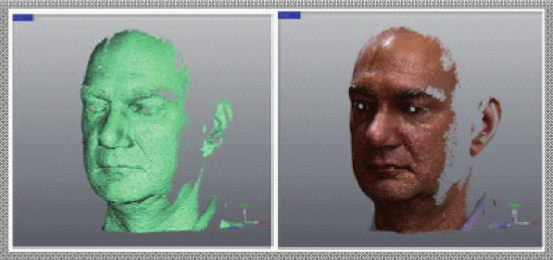
\includegraphics[scale=.35]{images/scans-3D}
\caption{Scans 3D \textit{sans} et \textit{avec} mapping de texture. Modèles issus de la base FRGCv2 \cite{Xphdthesis_4}}
\end{figure}\\
Les principales méthodes actuelles qui permettent la reconnaissance de visages en 3D sont les suivantes \cite{Xphdthesis_4}:
\begin{itemize}\setlength{\itemsep}{.2em}
\item[$\cdot$]Approches \textsc{\textbf{surfaces}}: la surface 3D du modèle reconstruit est alignée avec celle de la signature à comparer pour évaluer le taux de similitude par approximations.
\item[$\cdot$]Approches \textsc{\textbf{holistiques}} ou (\textsc{globales}): extensions des méthodes ACP 2D pour les représentations 3D, par exemple: \textit{eigensurface}.
\item[$\cdot$]Approches \textsc{\textbf{locales}}: cherches des courbes du visages ou des points caractéristiques
\item[$\cdot$]Approches \textsc{\textbf{3D + 2D}}: combinaisons de techniques d'analyse 3D et 2D pour améliorer les performances et la robustesse
\end{itemize}
\paragraph{}
La reconnaissance 3D comparée à la 2D permet d'obtenir de meilleurs résultats.
\\
De plus, les scans 3D sont beaucoup moins sensibles aux divers changements d’illumination, de variation de la pose ou encore de mise à l’échelle, autant de critères qui sont les éléments critiques de la reconnaissance automatique 2D.
\\
Toutefois, elle est plus difficile à mettre en place, consomme plus de ressources de calcul et nécessite l'utilisation de capteurs plus onéreux.

\subsection{Identification et authentification}\label{id-vs-auth}
Une fois la signature reconstruite à partir des données extraites de l'image, celle-ci va être comparée avec d'autres modèles. La validation se base sur un seuil du taux de similitudes entre les deux fichiers numériques.
\paragraph{}Dans le cas de l'identification, la signature peut être comparée avec l'ensemble des gabarits de la DB pour retrouver l'individu en question ou, dans une optique de recherches, elle peut être comparée avec seulementune liste de modèles pour détecter un éventuel match.
\paragraph{}Dans une utilisation d'authentification, une requête est faite vers la DB pour obtenir le modèle à comparer et vérifier si la signature reconstruite y correspond ou non.
\subsection{Mesure de la performance}
Afin d'évaluer les performances d'un système biométrique par reconnaissance de visage et pour aider la recherche et le développement de ces technologies, il existe des bases de données contenant de nombreux templates pouvant être utilisés. Ainsi, à titre d'exemple, il existe la base FERET, avec plusieurs centaines d'invidus collectés, ou la base XM2VTS qui contient un ensemble d'images faciales 2D et 3D avec différentes prises de vues \cite{Xphdthesis_3}.


\section{Exemples d'utilisation}
\textit{Les applications de la reconnaissance faciale sont nombreuses, depuis la sécurité des portiques d'aéoroports, jusqu'à la modélisation d'animation 3D en passant par ... }
\subsection{Les portails de sécurité dans les aéroports}
\subsection{La FaceID}
\subsection{Mais encore... quel futur pour la reconnaissance faciale}
\textcolor{dkblue}{\textit{Compte tenu des progrès fait en matière de reconnaissance faciale et de son intégration dans des systèmes tels que les smartphones, quelles applications pourrait-on envisager à l'avenir grâce à une telle technologie?}}
%\section{Les aspects liés à la sécurité}

\subsection{Impact par rapport aux anciens systèmes}
\subsection{Les risques potentiels}
\subsection{Législation}
\textit{En Europe, il est interdit de détcter les visages des gens sur les photos car cela peut mettre en péril leur vie privée - Exemple Facebook "DeepFace"}
\subsection{Questions éthiques... faut-il avoir "peur" de la reconnaissance faciale}
\textcolor{dkblue}{\textit{Les technologies biométriques stockent des informations très personnelles sur les individus comme ses empreintes digitales, ses données faciales, ... dès lors, cela soulève certaines questions quant à la protection de notre vie privée et la sécurité de ces informations. Il y a-t-il des risques potentiels à fournir tant de données à des "inconnus" , si oui lesquels? Dans quelles mesures peut-on accepter que des systèmes (sites, ) collectent autant de données sensibles à notre égard? Quelle serait-la prochaine étape?}}

\section{Conclusion}
Au fil de ces dernières décennies, les techniques de reconnaissance de visages se sont fortement améliorées proposant nombre de méthodes analysant des modèles 2D et 3D, avec des performances différentes et des dispositifs physiques plus ou moins onéreux. De plus, les nouvelles technologies ont permis de miniaturiser les capteurs de telle sorte que maintenant ils puissent même être embarqués dans des appareils mobiles.
\\Ces prouesses permettent ainsi d'obtenir des systèmes biométriques d'authentification de plus en plus performants qui améliorent la sécurité de nos appareils ou des mécanismes d'accès.
\\La reconnaissance de visages va également permettre à l'avenir de sécuriser des lieux publics, où circulent de nombreuses personnes, en traquant des suspects.
\\Toutefois, il est à noter que si les technologies biométriques représentent des solutions pratiques incontournables à l'heure du numérique et du "tout connecté", certains systèmes stockent des informations très personnelles sur les individus comme leurs empreintes digitales, leurs données faciales, leur comportement... Dès lors, cela peut soulever certaines questions quant à la protection de notre vie privée et la sécurité de ces informations. Il y a-t-il des risques potentiels à nous dévoiler autant à des "inconnus"? Serons-nous un jour contraints par les autorités de fournir l'ensemble de nos caratéristiques biométriques pour constituer des bases de données nationales? Dans quelle mesure peut-on accepter que des systèmes nous surveillent en public (\textit{"pour notre bien et la sécurité"})? Autant de questions pour lesquelles chacun à la liberté de se faire sa propre opinion mais probablement qu'il faudra un jour tout simplement accepter d'évoluer avec son temps et de profiter avant tout des bénéfices qu'offre ces nouvelles technologies, en échange de l'intrusion quelles occasionnent.

\bibliographystyle{unsrt}
\bibliography{biblio}

\appendix
\section{Evaluation du taux de performance des systèmes biométriques}
\begin{figure}[h!]
\center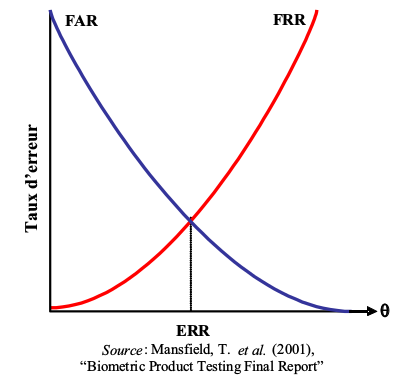
\includegraphics[scale=.5]{images/biometrie-performance}\label{perfo-systeme}
\caption{Source: \cite{Xphdthesis_1}}
\end{figure}
Les taux d'erreurs (\textit{Fausses Acceptations} et \textit{Faux Rejets}) dépendent du seuil de tolérance fixé. Les deux courbes varient de façon "opposée", de telle sorte que, par exemple, en diminuant le seuil de tolérance le match des signatures comparées soit plus vite validé, au risque d'augmenter le nombre d'individu faussement reconnus.  C'est l'intersection des courbes, le point TEE, qui est utilisé pour évaluer la performance d'un algorithme de reconnaissance par biométrie.

\section{Comparaison des méthodes locales et globales de reconnaissance 2D}
\begin{figure}[h!]
\center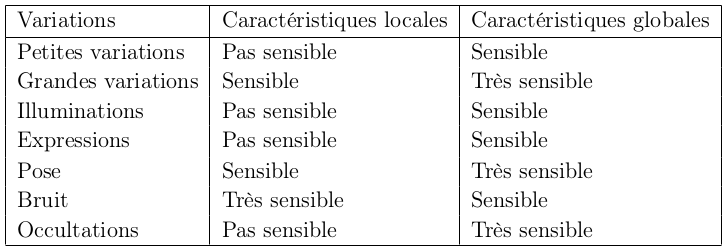
\includegraphics[scale=.4]{images/locales-vs-globales}\label{locales-vs-globales}
\caption{Tableau comparatif issu de \cite{Xphdthesis_1}}
\end{figure}

\end{document}
